\chapter{Bruit 5G}

Lorsqu'un appareil émet sur le spectre de la 5G à proximité du capteur QCM, les ondes émises peuvent interférer avec l'électronique de l'appareil de mesures, comme le montre la figure \ref{fig:bruit-5g}.
Cela peut fausser les mesures des fréquences de résonance et d'amplitude du capteur QCM.
Il est donc essentiel d'éloigner les appareils émettant sur ces fréquences tels que les téléphones afin de garantir la fiabilité et la précision des résultats obtenus.

\begin{figure}[H]
    \centering
    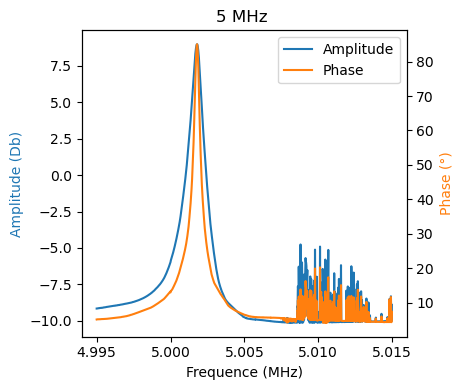
\includegraphics[width=0.8\textwidth]{assets/figures/bruit5G.png}
    \caption{Illustration du bruit 5G}
    \label{fig:bruit-5g}
\end{figure}

\chapter{Choix harmoniques}
\label{chap:choix_harmoniques}
Les mesures de fréquence et d'amplitude ont été faites sur trois harmoniques du quartz : la 1\up{re}, la 3\up{e} et la 5\up{e}.  
La 3\up{e} harmonique a été choisie pour les résultats lors du chapitre~\ref{chap:application_experimentale}, car elle présente le moins de bruit.  
La 1\up{re} et la 5\up{e} harmonique sont trop bruitées pour être utilisables.  

Voici un exemple de mesure avec de l'eau sur les trois harmoniques : on peut voir que la 3\up{e} est la plus stable.

\begin{figure}[H]
    \centering
    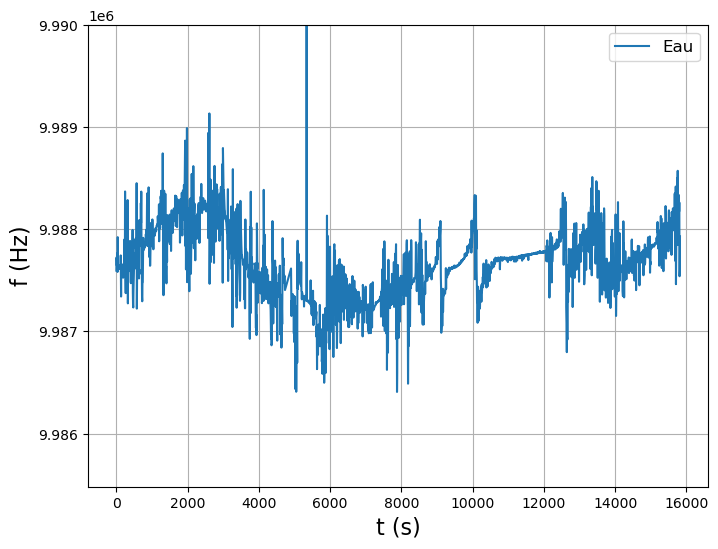
\includegraphics[width=0.8\textwidth]{assets/figures/annex10MHzFrequ.png}
    \caption{Mesure de la 1ère harmonique à 10Mhz avec de l'eau}
    \label{fig:choix_harmonique10MHz}
\end{figure}

\begin{figure}[H]
    \centering
    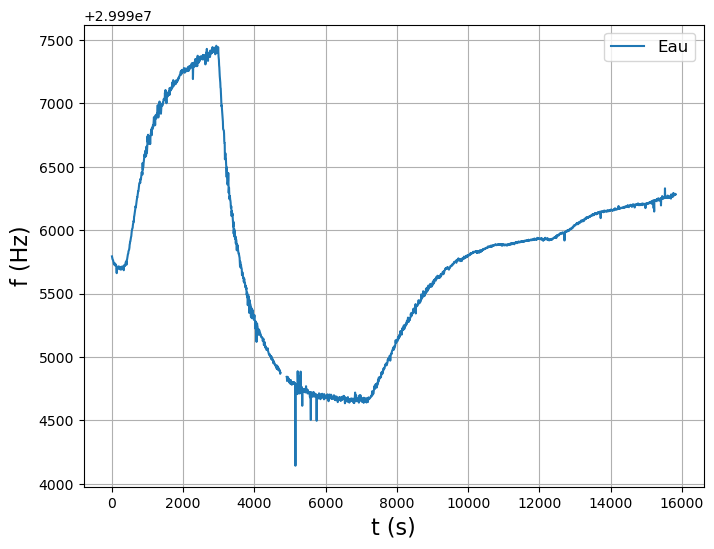
\includegraphics[width=0.8\textwidth]{assets/figures/annex30MHzFrequ.png}
    \caption{Mesure de la 3ème harmonique à 30Mhz avec de l'eau}
    \label{fig:choix_harmonique30MHz}
\end{figure}

\begin{figure}[H]
    \centering
    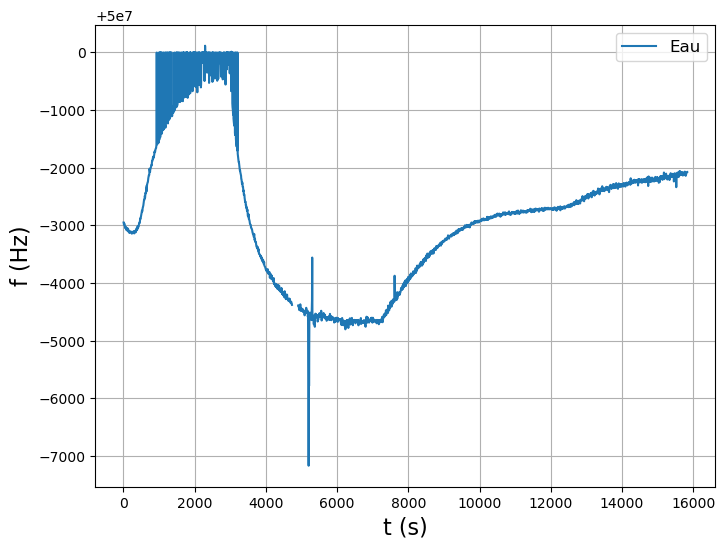
\includegraphics[width=0.8\textwidth]{assets/figures/annex50MHzFrequ.png}
    \caption{Mesure de la 5ème harmonique à 50Mhz avec de l'eau}
    \label{fig:choix_harmonique50MHz}
\end{figure}
\chapter{Manuel d'utilisation QCMApp}
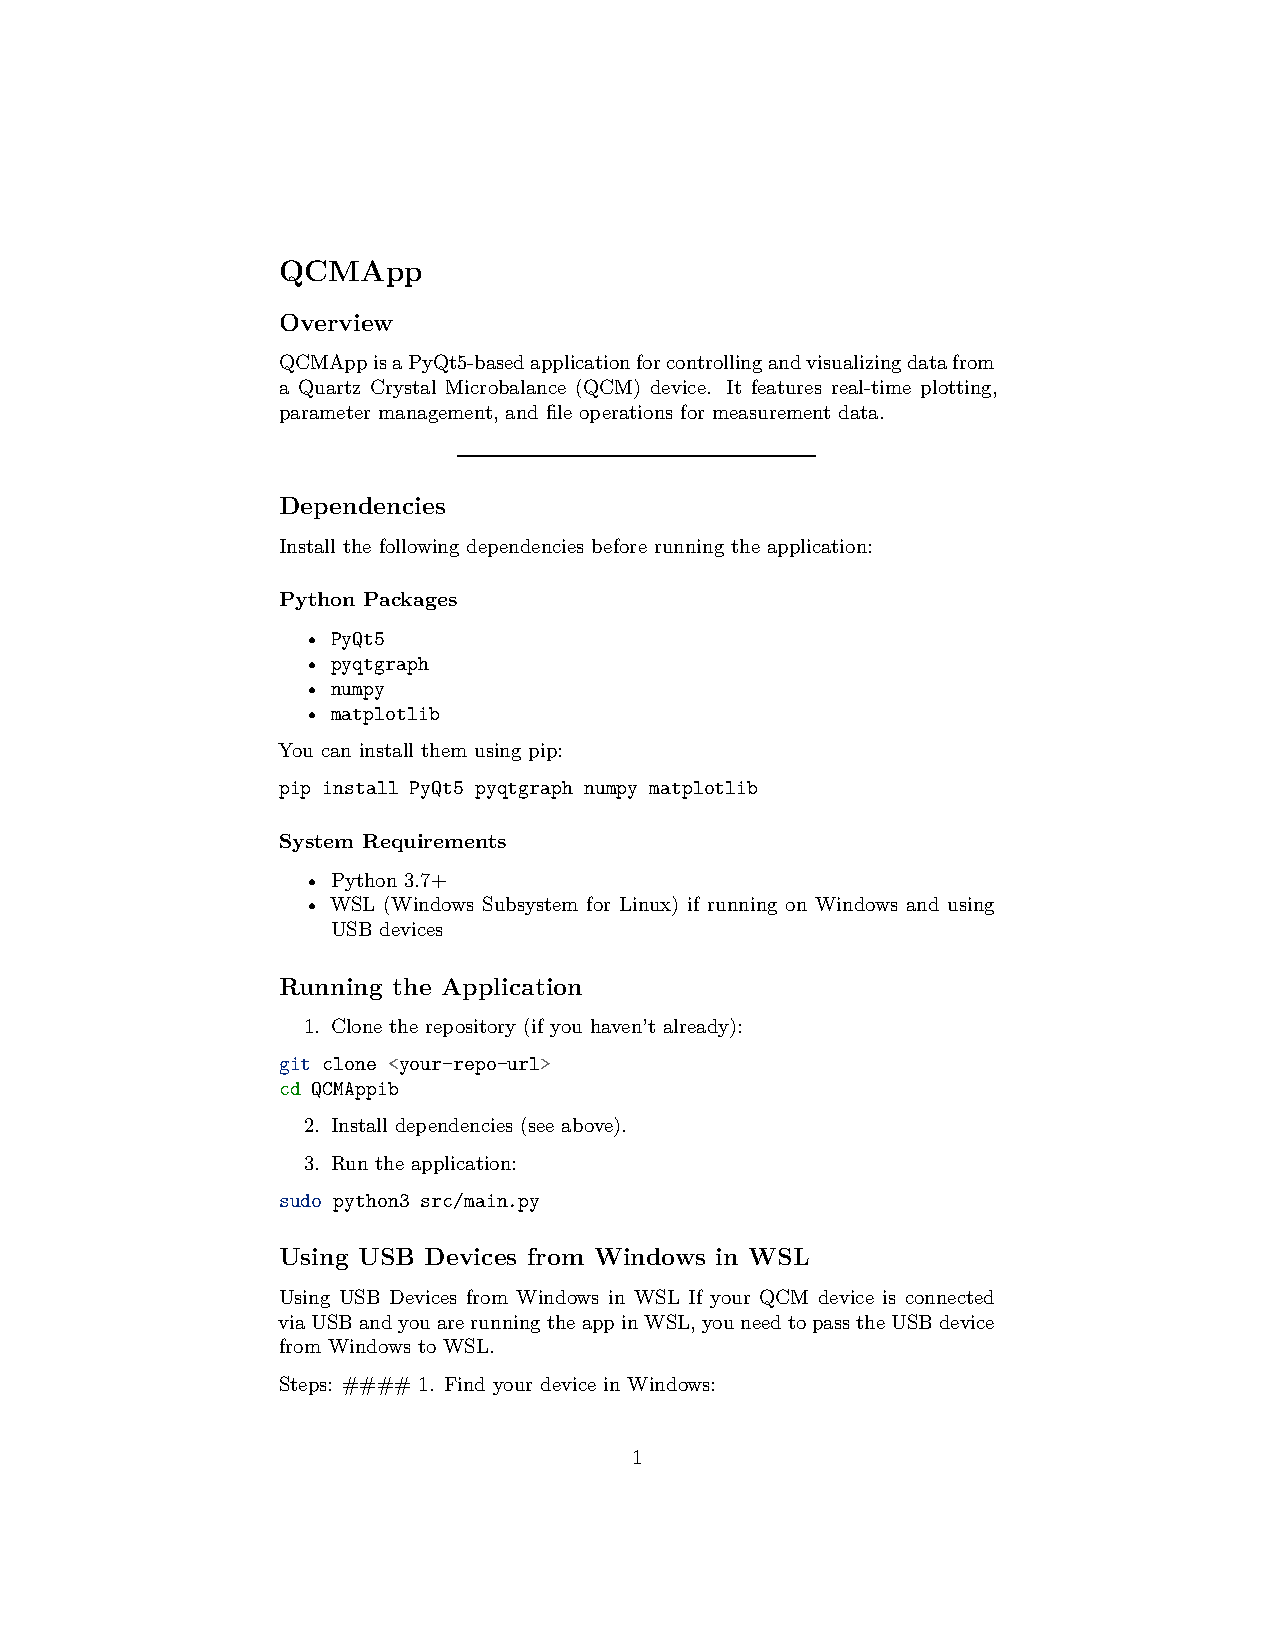
\includepdf[pages=-]{assets/readme.pdf}